\documentclass[main.tex]{subfiles}
\begin{document}
%TODO: remove active voice and replace with passive?
\chapter{Program Logic} 
	\section{Overview}
	The Atmega328p application program uses two processes to asynchronously
	control the external display and temperature conversion tasks (as shown in
	\figref{progLogic}).	Temperature calculations are handled by the ADC
	interrupt service routine (or ADC ISR). The ADC ISR obtains the result from
	the ADC and calls \lstinline{setTemp()} to handle temperature calculations.
	An eight-bit timer on the Atmega328p is used to manage the seven segment
	display.  Multiplexing is used to display a value on the and the
	\lstinline{setNum()} function is the application interface to set the number
	to display. 
	
	\begin{figure}[H]
		\begin{center}
			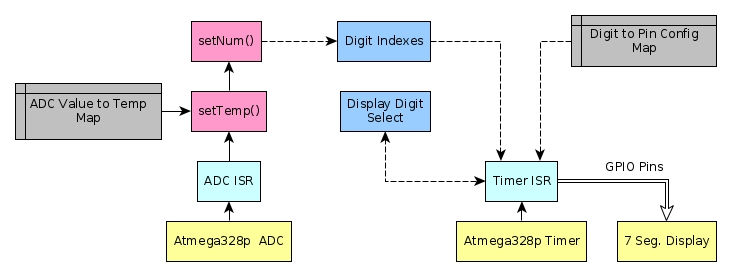
\includegraphics[width=\linewidth]{ProgramLogic}
		\end{center}
		\caption{Thermometer Program Logic}
		\label{fig:progLogic}
	\end{figure}

	\section{Configuration}
		\subsection{Timer Configuration}
		The eight-bit timer is configured to run at approximately fifty-two kilohertz
		in Clear Timer on Compare mode. CTC mode is an operation mode of the timer in
		which the internal counter is reset when the counter matches the value stored
		in the timer's output compare register. Once the timer is reset a timer
		interrupt vector flag is set and the timer ISR is called to handle the display.

		\subsection{ADC Configuration}
		The ADC is configured to run in Free running mode. This is an operation mode
		in which the ADC is constantly performing conversions. Once a conversion is
		performed an ADC flag is set and an interrupt is called and the ADC
		immediately begins performing another conversion. The ADC uses the
		\lstinline{ADC5} port as the voltage signal input. 

		\subsection{IO Register Configuration}
		\tabref{pinConfig} shows a table of specific ports and their
		respective pin configurations.

		\begin{table}[H]
			\begin{center}
				\begin{tabularx}{\textwidth}{llX} 
					Port & Pins & Configuration \\ \hline \hline
					PORTD & 0-7 & Output pins to control segment LEDs on seven-segment display. \\ \hline
					PORTC & 0-1 & Output pins to control digit selection on seven segment	display. \\ \hline
					PORTC & 5 & Input pin for ADC 
				\end{tabularx}
				\caption{Atmega328p Pin Configurations}
				\label{tab:pinConfig}
			\end{center}
		\end{table}
	
	\section{Two Digit Display}
		\begin{figure}[H]
			\begin{center}
				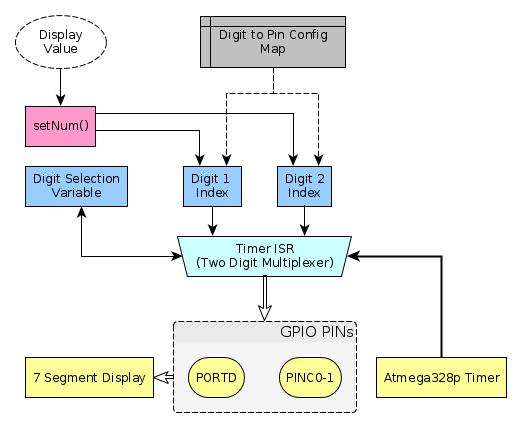
\includegraphics[width=\linewidth]{display}
			\end{center}
			\caption{Two Digit Display Interface}
			\label{fig:twoDigitIfc}
		\end{figure}
		\subsection{Single Digit Control}

		The two digit seven segment display is controlled by the Atmega328p via two
		I/O ports. \lstinline{PORTD} controls the segments on the display and
		\lstinline{PORTC} controls the digit selection. A mapping array is used to
		map digits 0 through 9 to their respective output register values. For
		example, the value at index 3 in the mapping array stores the respective
		value for the \lstinline{PORTD} register. This register value is then used
		to show the number 3 on the seven segment display. Two variables store
		indexes to this mapping array, each for a single digit on the display. These
		variables are set by the \lstinline{setNum()} function and are used by the
		timer ISR to set the \lstinline{PORTD} register. A variable is used to
		determine which digit to display when the ISR is called.
		\figref{twoDigitIfc} shows an overview of the display system.

		\subsection{Two Digit Multiplexing}
		To display a two digit number a multiplexing method is used. This is done by
		alternatively toggling each digit on the display so that only one digit is
		on for a given time period. When the digits are alternatively toggled at a
		frequency larger than 10kHz they appear as if they are displaying
		simultaneously. 

		The timer ISR handles the multiplexing of the two digits. Below is the
		process used in the timer ISR to perform two digit multiplexing: 

		\begin{enumerate}
			\item Turn currently displayed digit off.
			\item Select other digit to display using the digit selection variable.
			\item Turn selected digit on using the corresponding index variable.
		\end{enumerate}

	\section{ADC to Temperature Conversion}
	The Atmega328p has a ten bit successive approximation analog to digital
	converter (noted as ADC). Successive approximation is an analog to digital
	conversion method in which the input signal is constantly compared to the
	output of a guessed analog value. (see \figref{adcSA} for a simplified flow
	diagram of a successive approximation ADC.). After all n bits of the converter
	are set the ADC raises a conversion the ADC interrupt service routine (or ADC
	ISR) is called to handle temperature conversion (see the ADC to Temperature
	Conversion section below). 
	\begin{figure}[H]
		\begin{center}
			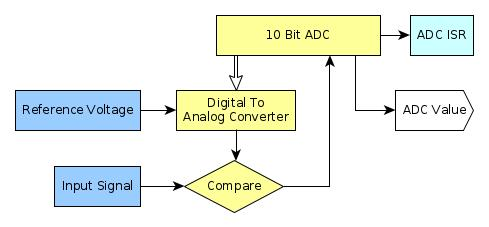
\includegraphics[width=\linewidth]{adc}
		\end{center}
		\caption{ADC Successive Approximation}
		\label{fig:adcSA}
	\end{figure}
	
		\subsection{Obtaining the ADC Conversion Result}
		\begin{figure}[H]
			\begin{center}
				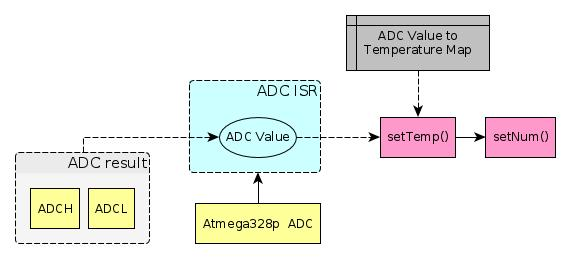
\includegraphics[width=\linewidth]{adcFlow}
			\end{center}
			\caption{Temperature Conversion Interface}
			\label{fig:tempConvIfc}
		\end{figure}

		The ADC uses two eight bit registers (called \lstinline{ADCL} and
		\lstinline{ADCH}) to store the result from an analog to digital conversion.
		The conversion result is obtained by fetching the \lstinline{ADCL} register
		data first (which is required according to the Atmega328p datasheet) and
		then the \lstinline{ADCH} register data. The final result is stored in a
		sixteen bit integer (noted as the ADC value) which is then passed to a
		temperature conversion function \lstinline{setTemp()}. \figref{tempConvIfc}
		shows the process in which the temperature conversion interface was
		designed.

		\subsection{Calculating the Temperature}
		%TODO: finish this section
		A function called \lstinline{setTemp()} handles the conversion of an ADC
		value to a temperature. Below is the process for which
		\lstinline{setTemp()} uses to convert and ADC value. 
	
		\begin{enumerate}
			\item Fetch nearest data points from Temperature conversion table.
			\item Perform linear interpolation using integer math to compute a
				temperature.
			\item call \lstinline{setNum()} to display the result to the seven segment
				display.
		\end{enumerate}	

		Linear interpolation was the method used to calculate temperatures based on
		given ADC values. See the below section for details on linear interpolation.

		\subsection{Linear Interpolation}
		Linear interpolation is a method of estimating function values from a table
		of known input and function values. The idea is that two points are chosen
		from the table (one greater than, one less than the desired value) and a
		linear equation is formed from those two points. Then the desired function value is
		found by `plugging in' a given input value into this function.

		%include graph of data
		\begin{figure}[H]
			\begin{center}
				\subfile{figures/adcTempGraph.tex}
			\end{center}
			\caption{Sample ADC value to Temperature Linear Interpolation}
			\label{gph:adcTempGraph}
		\end{figure}

		\gphref{adcTempGraph} shows an example of a linear interpolation. Each data
		point shown is a known ADC value and its corresponding temperature. The
		lines between each data point represent the functions to be used for linear
		interpolation.
		
		For example if the ADC value $400$ was returned by the ADC and one wished to
		know the corresponding temperature then one would find the two nearest
		points ($(343,20)$ and $(445,30)$) and create the line between the two
		and substitute the ADC value:

		\begin{eqnarray*}
			f(x) & = & \frac{(30-20)}{(445-343)}(x-343)+20 \\
			& \therefore & f(400) \approx 25.59^{\circ}\mathrm{C}
		\end{eqnarray*}

		A generic equation would be:

		\[
			f(x) = \frac{(y_{2}-y_{1})}{(x_{2}-x_{1})}(x-x_{1})+y_{1}\\
		\]

		where $(x_{1,2},y_{1,2})$ are two nearest points in the table surrounding a
		given ADC value $x_{n}$. 

\end{document}
